\section{主な機能}

\newcommand{\MyFunctionTable}[4]{
    \begin{frame}{機能要件}
        \begin{enumerate}
            \setbeamercovered{dynamic}
            \setlength{\itemsep}{0.8zh}
            \item<#1> 任意のコマンドラインを実行するたびに,その必要性を判断して,対応する命令をDockerfileに追加する機能
            \item<#2> CUI上でDockerfileを編集する機能
            \item<#3> ベストプラクティスに基づいて,作成されたDockerfileのリファクタリング・最適化を行う機能
            \item<#4> Dockerfileの開発を任意のタイミングで中断・再開できるようにする機能
        \end{enumerate}
    \end{frame}
}

\MyFunctionTable{1}{1}{1}{1}
\MyFunctionTable{1}{0}{0}{0}


\begin{frame}[fragile]{機能1\\「任意のコマンドラインを実行するたびに処理を行う」}
    Bashのシェル変数PROMPT\_COMMANDを使用する.
    \vskip2.0zh

    使用例
\begin{lstlisting}[language=sh]
# log each time the shell prompt is updated
PROMPT_COMMAND='mylog > "/tmp/$(date -Ins)"'
\end{lstlisting}

\end{frame}


\begin{frame}{機能1\\「変換仕様により,コマンドの反映の要否を判断する」}
    \begin{figure}
        \centering
        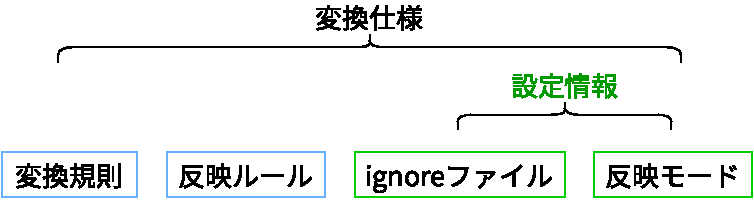
\includegraphics[width=\linewidth]{img/terms.pdf}
    \end{figure}
\end{frame}


\begin{frame}{機能1 変換規則の一覧}
    \small
    \begin{table}[h]
        \centering
        \begin{tabular}{c|c|l}
            変換前 & 変換後 & \multicolumn{1}{c}{備考} \\
            \hline\hline
            cd & WORKDIR命令 & 作業ディレクトリが変更された場合 \\
            pushd & & \\
            popd & & \\
            \hline
            代入文 & ARG命令 & コマンド実行環境を変更する場合 \\
            declare & & 左のコマンド以外には未対応 \\
            typeset & & \\
            readonly & & \\
            printf & & \\
            \hline
            export & ENV命令 & コマンド実行環境を変更する場合 \\
            & & ``declare -x''はARG命令に変換する \\
            \hline
            それ以外 & RUN 命令 & 複数に変換されることはない\\
        \end{tabular}
    \end{table}
\end{frame}


\begin{frame}{機能1 デフォルトの反映ルール(一部抜粋)}
    \small
    \begin{table}[h]
        \centering
        \begin{tabular}{c|l}
            Bashの構文 & \multicolumn{1}{c}{反映ルール} \\
            \hline\hline
            単純なコマンド & 出力のリダイレクションを含む場合は反映する \\
            算術式 & letに対するignoreファイルの設定を使う \\
            条件式 & 単独で使われた場合は反映しない \\
            パイプライン & 反映するコマンドより左にあるものは反映する \\
            条件付きリスト & 反映するコマンドを含む場合,まとめて反映する \\
            その他のリスト & 各コマンドの反映の要否を個別に決定する \\
        \end{tabular}
    \end{table}

    \vskip1.0zh
    \textreferencemark 後述の反映モードの設定により,内容が少し変動する.
\end{frame}


\begin{frame}[fragile]{機能1 ignoreファイルの例}
    反映しないコマンドとその条件を記述する.
\begin{lstlisting}[language=json]
{
    "ls": null,
    "dir": "ls",
    "wget": {
        "short_opts": "O:",
        "long_opts": {
            "output-document": 1
        },
        "optargs": {
            "output-document": "O",
            "O": [
                "-"
            ]
        },
        "detect_anymatch": true
    }
}
\end{lstlisting}

\end{frame}


\begin{frame}{機能1 反映モードの一覧}
    \begin{description}
        \item[no-reflect] Dockerfileに命令を追加しない
        \item[strict] 処理の流れに影響しない部分は特別視しない
        \item[normal] 処理のまとまりを考え,反映の要否を変更する
        \item[simple] 単純なコマンド\footnote{Bashの基本構文.}以外はそのまま反映する
        \item[no-ignore] 実行されたコマンドラインは必ず反映する
    \end{description}

    \vskip1.0zh
    \textcolor{red!75}{strictとnormalの違い}(例:条件実行の``left \&\& right'')
    \begin{description}
        \item[strict] 左のコマンドだけを反映する可能性がある
        \item[normal] ひとまとめに反映するか,全く反映しないか
    \end{description}
\end{frame}


\begin{frame}{機能1 変換処理の流れ}
    \begin{tikzpicture}[remember picture]
        \useasboundingbox (0.0, 0.0);
        \begin{scope}[shift={(current page.south west)}]
            \node[progress20] (p1) at (6.8, 7.6) {直前の終了ステータスを判定};
            \node[progress20] (p2) at (6.8, 6.4) {現在の反映モードを判定};
            \node[progress20] (p3) at (6.8, 5.2) {コマンドラインを解析・展開};
            \node[progress10] (p4) at (2.2, 4.0) {変換規則の適用};
            \node[progress20] (p5) at (6.8, 2.8) {ignoreファイル・反映ルールの適用};

            \node[success] (g1) at (2.2, 1.0) {対応する命令を追加};
            \node[success] (g2) at (6.8, 1.0) {RUN命令を追加};
            \node[failure] (g3) at (11.4, 1.0) {失敗で終了};

            \coordinate (c1) at (2.2, 2.8);
            \coordinate (c2) at (6.8, 4.0);
            \coordinate (c3) at (11.4, 2.8);
            \coordinate (c4) at (11.4, 6.4);
            \coordinate (c5) at (11.4, 7.6);

            \foreach \u / \v in {p1/p2,p2/p3,p3/p5,p4/g1,p5/g2,c1/p5,c2/p4}
                \draw[arrows = {-Stealth}] (\u) -- (\v);

            \foreach \u / \v in {p1/c5,p2/c4,p5/c3,c5/g3}
                \draw[red, arrows = {-Stealth}] (\u) -- (\v);

            \begin{tikzpicture}[remember picture, overlay]
                \only<2>{\node[callout, callout absolute pointer={(p2.north)}] at (1.2, 3.0) {成功ならば};}
                \only<3>{\node[callout, callout absolute pointer={(p3.north)}] at (1.2, 1.8) {no-reflect以外};}
                \only<4>{\node[callout, callout absolute pointer={(p4.east)}] at (1.2, 1.0) {候補にだけ};}
                \only<5>{\node[callout, callout absolute pointer={(c3)}] at (7.2, 0.0) {反映するものがなければ};}
            \end{tikzpicture}
        \end{scope}
    \end{tikzpicture}
\end{frame}


\begin{frame}[fragile]{機能1 変換処理の具体例}
    \begin{figure}
        \centering
        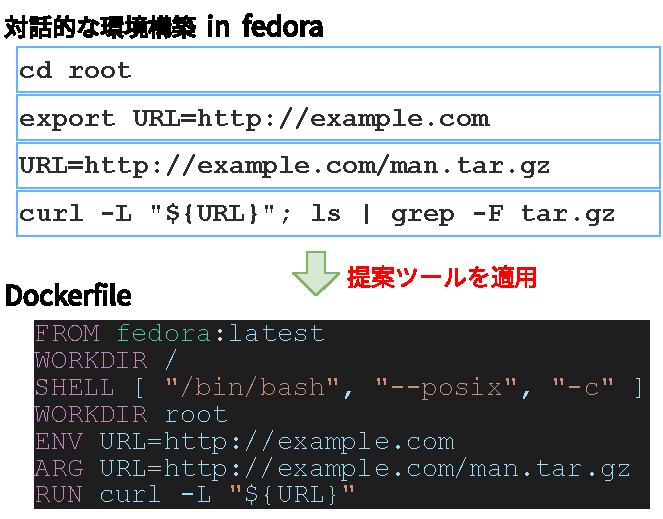
\includegraphics[width=\linewidth]{img/convert.pdf}
    \end{figure}
\end{frame}




\MyFunctionTable{0}{1}{0}{0}


\begin{frame}{機能2\\「ホスト環境からファイルをコピーする」}
    \textcolor{blue!75}{dit copy}

    \hskip1.0zw
    ホスト環境からコンテナ内へのファイルのコピーを行い,その内容をCOPY・ADD命令としてDockerfileに反映する.
    \vskip2.0zh

    このコマンドを使うと,
    \begin{itemize}
        \item COPY命令とcpコマンドの仕様の違いを意識せず済む.
        \item ADD命令のtar展開機能を利用できる.
    \end{itemize}
\end{frame}


\begin{frame}{機能2\\「パッケージをインストールする」}
    \textcolor{blue!75}{dit package}

    \hskip1.0zw
    最適化された形式で,パッケージのインストールを行い,その内容をRUN命令としてDockerfileに反映する.
    \vskip2.0zh

    このコマンドを使うと,
    \begin{itemize}
        \item イメージサイズの削減に効果的な方法で実行される.
        \item パッケージマネージャの違いをあまり意識せず済む.
    \end{itemize}
\end{frame}


\begin{frame}[fragile]{機能2\\「Dockerfileに命令を追加する」}
    \textcolor{blue!75}{dit reflect}

    \hskip1.0zw
    各種ログを取りながら,Dockerfileに命令を追加する.
    \vskip1.0zh
    実行例

\begin{lstlisting}[language=sh]
# reflects the contents of `./instr.txt' in Dockerfile
dit reflect -d instr.txt
\end{lstlisting}

\begin{lstlisting}[language=sh]
# reflects the input contents as they are in Dockerfile
dit reflect -dp -
\end{lstlisting}

\end{frame}


\begin{frame}[fragile]{機能2\\「Dockerfileから指定した行を削除する」}
    \textcolor{blue!75}{dit erase}

    \hskip1.0zw
    条件にマッチする行を,Dockerfileから削除する.
    \vskip1.0zh
    実行例

\begin{lstlisting}[language=sh]
# deletes the lines added just before from Dockerfile
dit erase -d
\end{lstlisting}

\begin{lstlisting}[language=sh]
# deletes all LABEL instructions from Dockerfile
dit erase -diy -E '^LABEL[[:space:]]'
\end{lstlisting}

\end{frame}




\MyFunctionTable{0}{0}{1}{0}


\begin{frame}{機能3\\「Dockerfileのリファクタリング・最適化を行う」}
    \textcolor{blue!75}{dit optimize}

    \hskip1.0zw
    下書きのDockerfileから,完成版のDockerfileを生成する.
    \vskip1.0zh

    処理内容の例
    \begin{itemize}
        \item WORKDIR命令のオペランドを絶対パスにする.
        \item 重複した命令など,無意味な命令を取り除く.
        \item 連続するRUN命令をまとめる.
        \item 可読性を向上させるための整形を行う.
    \end{itemize}
\end{frame}




\MyFunctionTable{0}{0}{0}{1}


\begin{frame}{機能4\\「Dockerfileの開発を中断・再開できるようにする」}
    コマンドラインの実行履歴を保持する,\textcolor{red!75}{履歴ファイル}\\を導入することで実現する.

    \vskip1.0zh
    \begin{description}
        \setlength{\itemsep}{1.0zh}
        \setlength{\leftskip}{-1.0zw}
        \item[開発中] Dockerfileと同じように履歴ファイルを編集する.
        \item[再開時] 履歴ファイルを実行して,環境を再現する.
    \end{description}
\end{frame}